% Created 2025-07-20 Sun 17:15
% Intended LaTeX compiler: pdflatex
\documentclass[11pt]{article}
\usepackage[utf8]{inputenc}
\usepackage[T1]{fontenc}
\usepackage{graphicx}
\usepackage{longtable}
\usepackage{wrapfig}
\usepackage{rotating}
\usepackage[normalem]{ulem}
\usepackage{amsmath}
\usepackage{amssymb}
\usepackage{capt-of}
\usepackage{hyperref}
\usepackage{minted}
\usepackage[a4paper]{geometry}
\usepackage{mathtools}
\author{Alexander Huss}
\date{\today}
\title{\(\mathrm{e}^+\mathrm{e}^- \to \mu^+ \mu^-\)}
\hypersetup{
 pdfauthor={Alexander Huss},
 pdftitle={\(\mathrm{e}^+\mathrm{e}^- \to \mu^+ \mu^-\)},
 pdfkeywords={},
 pdfsubject={},
 pdfcreator={Emacs 30.1 (Org mode 9.7.31)}, 
 pdflang={English}}
\usepackage{biblatex}

\begin{document}

\maketitle
\tableofcontents

\section{Introduction}
\label{sec:org256b156}
We will implement the process \(\mathrm{e}^+\mathrm{e}^- \to \mu^+ \mu^-\) at leading order.
This is among the simplest processes there are but it gives us many knobs to play around with to get an idea about the physics underlying these predictions.
\section{Cross section and forward--backward asymmetry}
\label{sec:orgb38ad48}

\subsection{The squared Matrix Element}
\label{sec:org5182538}
We have seen in the lecture that the squared amplitude (summed/averaged over final-/initial-state degrees of freedom) is given by
\begin{align}
  \frac{1}{4} \sum_\text{spins}
  \bigl\lvert \mathcal{M}_\gamma + \mathcal{M}_\mathrm{Z} \bigr\rvert^2
  &=
  e^4 \Bigl[ G_1(s)\; (1+\cos^2(\theta)) + G_2(s)\; 2 \cos(\theta) \Bigr]
\end{align}
with the functions
\begin{align*}
  G_1(s) &=
  1
  + 2 v_\mathrm{e} v_\mu \mathrm{Re}\biggl\{\frac{s}{s - M_\mathrm{Z}^2 + \mathrm{i}\Gamma_\mathrm{Z}M_\mathrm{Z}}\biggr\}
  + (v_\mathrm{e}^2 + a_\mathrm{e}^2) (v_\mu^2 + a_\mu^2) \biggl\lvert\frac{s}{s - M_\mathrm{Z}^2 + \mathrm{i}\Gamma_\mathrm{Z}M_\mathrm{Z}}\biggr\rvert^2
  \\
  G_2(s) &=
  0
  + 2 a_\mathrm{e} a_\mu \mathrm{Re}\biggl\{\frac{s}{s - M_\mathrm{Z}^2 + \mathrm{i}\Gamma_\mathrm{Z}M_\mathrm{Z}}\biggr\}
  + 4 v_\mathrm{e} a_\mathrm{e} v_\mu a_\mu \biggl\lvert\frac{s}{s - M_\mathrm{Z}^2 + \mathrm{i}\Gamma_\mathrm{Z}M_\mathrm{Z}}\biggr\rvert^2
\end{align*}
\subsubsection{Implementation}
\label{sec:org036fcad}
We'll use a simple class to save and retrieve Standard Model parameters including some convenience functions:
\begin{minted}[frame=lines,fontsize=\scriptsize]{python}
class Parameters(object):
    """very simple class to manage Standard Model Parameters"""

    #> conversion factor from GeV^{-2} into nanobarns [nb]
    GeVnb = 0.3893793656e6

    def __init__(self, **kwargs):
        #> these are the independent variables we chose:
        #>  *  sw2 = sin^2(theta_w) with the weak mixing angle theta_w
        #>  *  (MZ, GZ) = mass & width of Z-boson
        self.sw2 = kwargs.pop("sw2", 0.223)
        self.MZ  = kwargs.pop("MZ", 91.1876)
        self.GZ  = kwargs.pop("GZ", 2.4952)
        if len(kwargs) > 0:
            raise RuntimeError("passed unknown parameters: {}".format(kwargs))
        #> let's store some more constants (l, u, d = lepton, up-quark, down-quark)
        self.Ql = -1.;
        self.I3l = -1./2.;
        self.alpha = 1./137.
        #> and some derived quantities
        self.sw = math.sqrt(self.sw2)
        self.cw2 = 1.-self.sw2  # cos^2 = 1-sin^2
        self.cw = math.sqrt(self.cw2)
    #> vector & axial-vector couplings to Z-boson
    @property
    def vl(self) -> float:
        return (self.I3l-2*self.Ql*self.sw2)/(2.*self.sw*self.cw)
    @property
    def al(self) -> float:
        return self.I3l/(2.*self.sw*self.cw)
    #> the Z-boson propagator
    def propZ(self, s: float) -> complex:
        return s/(s-complex(self.MZ**2,self.GZ*self.MZ))
#> we immediately instantiate an object (default values) in global scope
PARAM = Parameters()
\end{minted}
We next implement the functions \(G_1\) and \(G_2\) that were introduced to express the squared Matrix Element in terms of the even and odd components w.r.t. \(\cos(\theta)\):
\begin{minted}[frame=lines,fontsize=\scriptsize]{python}
def G1(s: float, par=PARAM) -> float:
  return par.Ql**2 - 2. * par.vl**2 * par.Ql * par.propZ(s).real + (par.vl**2 + par.al**2)**2 * abs(par.propZ(s))**2
def G2(s: float, par=PARAM) -> float:
  return -2. * par.al**2 * par.Ql * par.propZ(s).real + 4. * par.vl**2 * par.al**2 * abs(par.propZ(s))**2
\end{minted}
\subsection{Differential and total cross sections and \(A_{FB}\)}
\label{sec:org62d56a2}
The formula for the differential cross section reads
\begin{align}
  \frac{\mathrm{d}\sigma}{\mathrm{d}\cos\theta}
  &=
  \frac{\alpha^2\pi}{2 s} \Bigl[ G_1(s)\; (1+\cos^2(\theta)) + G_2(s)\; 2 \cos(\theta) \Bigr]
  \,,
\end{align}
where \(s=(p_{\mathrm{e}^+}+p_{\mathrm{e}^-})^2=(p_{\mu^+}+p_{\mu^-})^2 = 4 E_\mathrm{cm}^2\) is the centre-of-mass energy of the collision and \(\theta\) the scattering angle between the electron and the muon.

We obtain the total cross section by integrating over \(\cos\theta\):
\begin{align}
  \sigma
  &=
  \int_{-1}^{+1}\mathrm{d}\cos\theta \; \frac{\mathrm{d}\sigma}{\mathrm{d}\cos\theta}
  = \frac{\alpha^2\pi}{2 s} \; \frac{8}{3} \; G_1(s)
  \,.
\end{align}

Another interesting quantity to look at is the forward--backward asymmetry defined as:
\begin{align}
  A_{FB}
  &=
  \frac{1}{\sigma}\;\biggl\{
  \int_{0}^{+1}\mathrm{d}\cos\theta \; \frac{\mathrm{d}\sigma}{\mathrm{d}\cos\theta} -
  \int_{-1}^{0}\mathrm{d}\cos\theta \; \frac{\mathrm{d}\sigma}{\mathrm{d}\cos\theta}
  \biggr\}
  = \frac{3}{4} \; \frac{G_2(s)}{G_1(s)}
  \,.
\end{align}
\subsubsection{Implementation}
\label{sec:orga99e845}
We'll start with the implementation of the total cross section
\begin{minted}[frame=lines,fontsize=\scriptsize]{python}
def cross(s: float, par=PARAM) -> float:
  return par.GeVnb * par.alpha**2*math.pi/(2.*s) * (8./3.) * G1(s, par)
\end{minted}
and define another function for the forward-backward asymmetry
\begin{minted}[frame=lines,fontsize=\scriptsize]{python}
def AFB(s: float, par=PARAM) -> float:
  return (3./4.) * G2(s,par)/G1(s,par)
\end{minted}
\section{Playground}
\label{sec:orgc047fb3}

\subsection{Export source code}
\label{sec:orgce627c8}
We can export the python source code to a file \texttt{main.py}
\begin{minted}[frame=lines,fontsize=\scriptsize]{python}
import math
import cmath
import numpy as np
class Parameters(object):
    """very simple class to manage Standard Model Parameters"""

    #> conversion factor from GeV^{-2} into nanobarns [nb]
    GeVnb = 0.3893793656e6

    def __init__(self, **kwargs):
        #> these are the independent variables we chose:
        #>  *  sw2 = sin^2(theta_w) with the weak mixing angle theta_w
        #>  *  (MZ, GZ) = mass & width of Z-boson
        self.sw2 = kwargs.pop("sw2", 0.223)
        self.MZ  = kwargs.pop("MZ", 91.1876)
        self.GZ  = kwargs.pop("GZ", 2.4952)
        if len(kwargs) > 0:
            raise RuntimeError("passed unknown parameters: {}".format(kwargs))
        #> let's store some more constants (l, u, d = lepton, up-quark, down-quark)
        self.Ql = -1.;
        self.I3l = -1./2.;
        self.alpha = 1./137.
        #> and some derived quantities
        self.sw = math.sqrt(self.sw2)
        self.cw2 = 1.-self.sw2  # cos^2 = 1-sin^2
        self.cw = math.sqrt(self.cw2)
    #> vector & axial-vector couplings to Z-boson
    @property
    def vl(self) -> float:
        return (self.I3l-2*self.Ql*self.sw2)/(2.*self.sw*self.cw)
    @property
    def al(self) -> float:
        return self.I3l/(2.*self.sw*self.cw)
    #> the Z-boson propagator
    def propZ(self, s: float) -> complex:
        return s/(s-complex(self.MZ**2,self.GZ*self.MZ))
#> we immediately instantiate an object (default values) in global scope
PARAM = Parameters()
def G1(s: float, par=PARAM) -> float:
  return par.Ql**2 - 2. * par.vl**2 * par.Ql * par.propZ(s).real + (par.vl**2 + par.al**2)**2 * abs(par.propZ(s))**2
def G2(s: float, par=PARAM) -> float:
  return -2. * par.al**2 * par.Ql * par.propZ(s).real + 4. * par.vl**2 * par.al**2 * abs(par.propZ(s))**2
def cross(s: float, par=PARAM) -> float:
  return par.GeVnb * par.alpha**2*math.pi/(2.*s) * (8./3.) * G1(s, par)
def AFB(s: float, par=PARAM) -> float:
  return (3./4.) * G2(s,par)/G1(s,par)
if __name__ == "__main__":
    res = []
    for Ecm in np.linspace(20, 100, 200):
        s = Ecm**2
        xs = cross(s)
        afb = AFB(s)
        print("{:e} {:e} {:e}".format(Ecm,xs,afb))
\end{minted}
by using the \texttt{tangle} command
\begin{minted}[frame=lines,fontsize=\scriptsize]{elisp}
(org-babel-tangle)
\end{minted}
\subsection{Collider energy scan}
\label{sec:org55dc294}
Let's execute the python script we just exported and look at the total cross section and the forward--backward asymmetry as a function of the collider energy.
\begin{minted}[frame=lines,fontsize=\scriptsize]{shell}
python main.py
\end{minted}

\begin{center}
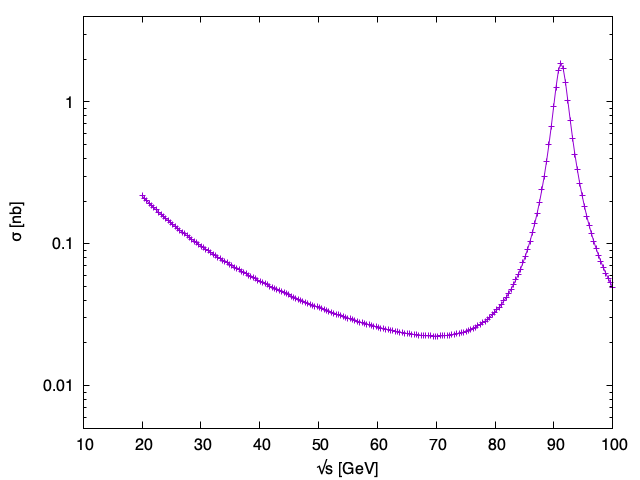
\includegraphics[width=.9\linewidth]{sigma.png}
\label{}
\end{center}


\begin{center}
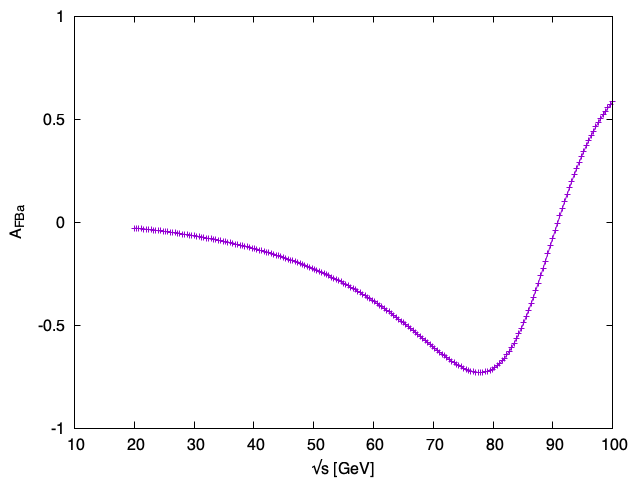
\includegraphics[width=.9\linewidth]{AFB.png}
\label{}
\end{center}
\subsection{\(M_\mathrm{Z}\) variation}
\label{sec:orga22d9b5}
Let's see how the cross section behaves under variation of the Z-boson mass
\begin{minted}[frame=lines,fontsize=\scriptsize]{python}
import math
import cmath
import numpy as np
<<util>>
<<cross>>
res = []
MZ_scan = [ Parameters(MZ=val) for val in [89, 90, 91, 92, 93] ]
for Ecms in np.linspace(80, 100, 50):
    s = Ecms**2
    ires = [Ecms.item()]
    for par in MZ_scan:
        xs = cross(s, par)
        ires.append(xs.item())
    res.append(ires)
return res
\end{minted}
let's plot the dependence on the Z-boson mass around the resonance
\begin{center}
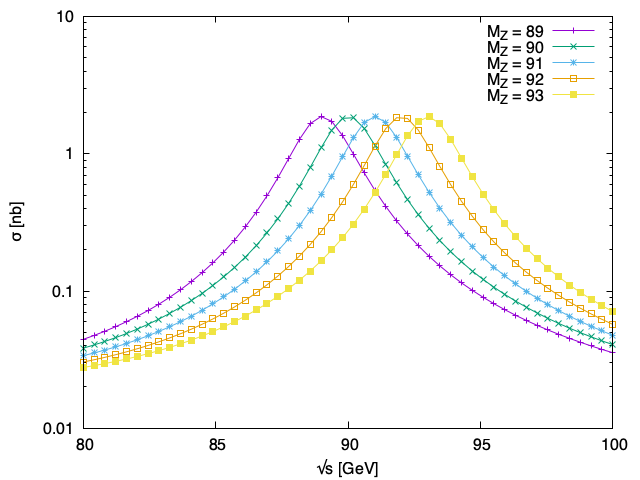
\includegraphics[width=.9\linewidth]{MZ_var.png}
\label{}
\end{center}
\subsection{\(\Gamma_\mathrm{Z}\) variation}
\label{sec:orgb397050}
Let's check how the picture would change if we had a different number of light neutrino species.
The branching fraction of a Z-boson decay into neutrino (``invisible decay'') is 20\%.
\begin{minted}[frame=lines,fontsize=\scriptsize]{python}
import math
import cmath
import numpy as np
<<util>>
<<cross>>
res = []
#> the partial decay width for Z -> massless (anti-)neutrino
GZ_nu = 0.2 * PARAM.GZ / 3.
GZ_scan = [ Parameters(GZ=PARAM.GZ-GZ_nu), PARAM, Parameters(GZ=PARAM.GZ+GZ_nu) ]
for Ecms in np.linspace(85, 95, 50):
    s = Ecms**2
    ires = [Ecms.item()]
    for par in GZ_scan:
        xs = cross(s, par)
        ires.append(xs.item())
    res.append(ires)
return res
\end{minted}
let's plot how much the Z line shape varies with the number of neutrino generations
\begin{center}
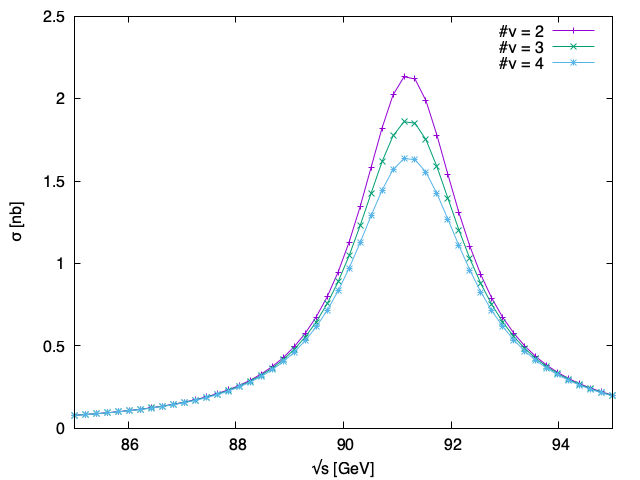
\includegraphics[width=.9\linewidth]{GZ_var.png}
\label{}
\end{center}
\subsection{\(A_{FB}\) and the weak mixing angle}
\label{sec:org4d8b1a2}
The forward--backward asymmetry is an observable that is sensitive to the weak mixing angle as we will see in the following.
Moreover, defined as a ratio, many systematic uncertainties cancel.
\begin{minted}[frame=lines,fontsize=\scriptsize]{python}
import math
import cmath
import numpy as np
<<util>>
<<cross>>
res = []
#> the partial decay width for Z -> massless (anti-)neutrino
sw2_step = PARAM.sw2 * 0.1  # 10% variation per step
sw2_scan = [ Parameters(sw2=PARAM.sw2+i*sw2_step) for i in [-3,-2,-1,0,1,2,3] ]
for Ecms in np.linspace(85, 95, 50):
    s = Ecms**2
    ires = [Ecms.item()]
    for par in sw2_scan:
        afb = AFB(s, par)
        ires.append(afb.item())
    res.append(ires)
return res
\end{minted}
let's see how much \(A_{FB}\) varies with \(\sin^2\theta_w\):
\begin{center}
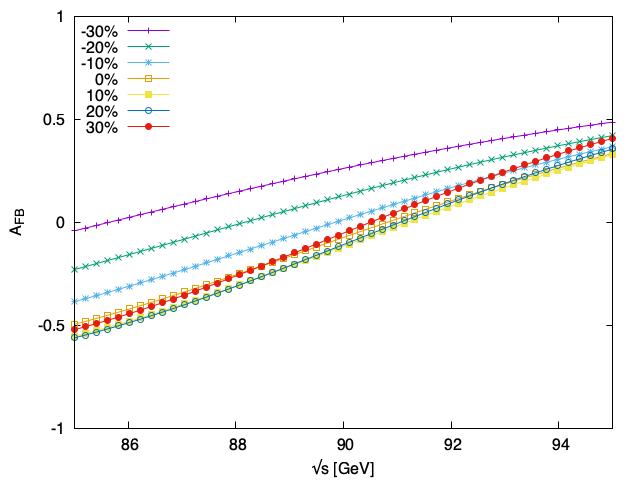
\includegraphics[width=.9\linewidth]{sw_var.png}
\label{}
\end{center}
\end{document}
